% \documentclass[xetex,mathserif,serif]{beamer}

\usepackage{tabu}

\AtBeginSection[]
{
    \begin{frame}
        \sectionpage
    \end{frame}
}

\begin{document}

\frame{\titlepage}

\begin{frame}
    \frametitle{Introduction}
    \begin{itemize}
        \item<1-> "Golden Age of Exoplanets"
        \item<2-> Statistics, signal processing, and Python
        \item<3-> Compare with accepted values
        \note[item]<1>{Kepler's found a bunch, lot of publicity, lot of potential methods}
        \note[item]<2>{Statistics - figure out what's important and significant, signal processing - find patterns, Python - lots of data points}
    \end{itemize}

    \begin{block}<4->{Hypothesis}
        If Kepler light curves for single-planet systems are analyzed using a straighforward implementation of basic exoplanet dectection methods, then
        the calculated parameters should correspond to the accepted values determined by more advanced transit and radial-velocity analysis.
    \end{block}
    \note<4->{Basically, I want to see how exoplanets are found and how close I can get with fairly simple stuff}
\end{frame}

\section{Background}

\begin{frame}
    \frametitle{Overview}
    \begin{itemize}
        \item<1-> "Hot Jupiters"
        \item<2-> Challenges
        \item<3-> Methods
        \item<4-> Kepler
        \note[item]<1>{Hot Jupiters - a few stellar radii away, orbital period of a couple days (Mercury is 88), 1-2 thousand Kelvin}
        \note[item]<2>{planets are dim and far away, stars are bright and bigger}
        \note[item]<3>{Doppler, transit, gravitational microlensing (planet gravity focuses star light -> brighter), direct imagin}
        \note[item]<4>{survey single region w/ a photometer over several years - transit method}
    \end{itemize}
\end{frame}

\begin{frame}
    \frametitle{The Radial Velocity Method}
    \begin{itemize}[<+->]
        \item Planet and star orbit center of mass
        \item Motion leads to Doppler shift in light
        \item Absorption lines shifted from reference values
    \end{itemize}
    \only<4->{
        \begin{align*}
            \lambda_{shift} = \lambda_{rest} \times \frac{v_{radial}}{c}
        \end{align*}
    }
\end{frame}

\begin{frame}
    \begin{figure}
        \centering
        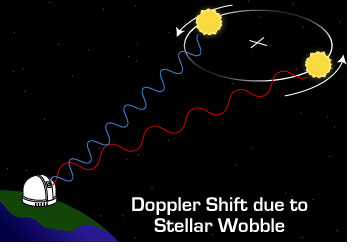
\includegraphics[height=0.8\textheight]{images/doppler1}
        \caption{Periodic pattern indicates a planet.}
    \end{figure}
\end{frame}

\begin{frame}
    \frametitle{The Transit Method}
    \begin{itemize}[<+->]
        \item Drop in apparent brightness of host star
        \item Observe many at once
        \item Light curves and periodograms
        \note{Looking for tiny decrease in brightness when the planet is between us and the star}
        \note{like an eclipse}
        \note{Kepler found around 1,000 exoplanet candidates}
        \note{Plot flux (change in intensity) against time}
        \note{BLS, Fourier, Lomb-Scargle, etc. - look for periodic patterns}
        \note{use BLS since it accounts for the transit shape - flat bottom every now and then}
    \end{itemize}
\end{frame}

\begin{frame}
    \begin{figure}
        \centering
        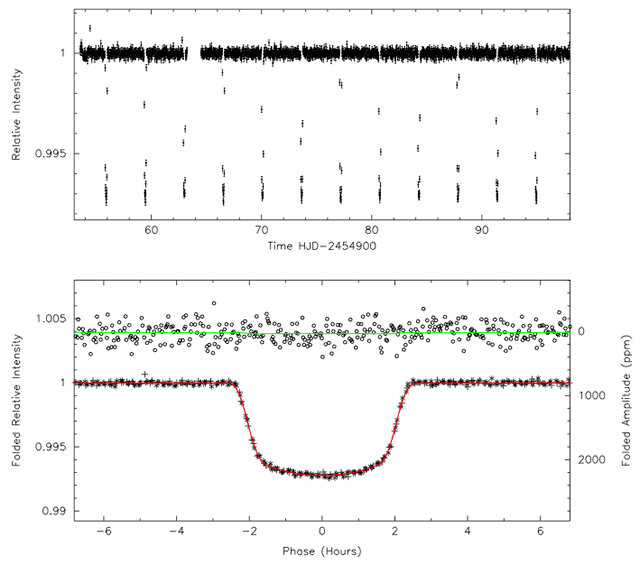
\includegraphics[width=0.7\textwidth]{images/lightcurve5b}
        \caption{Light curve for Kepler-5b and folded curve showing transit}
    \end{figure}
\end{frame}

\section{Procedure}

\begin{frame}
    \frametitle{Materials}
    \begin{itemize}
        \item<1-> Light curves for each planet of interest
        \item<2-> Analysis tools
        \note[item]<1>{Light curves can be pre-prepared, i.e. from Kepler, or generated from images, which could also be from Kepler or another telescope}
        \note[item]<2>{can have 100s or 1000s of data points, don't want to do everything by hand. Humans can be better at finding and tuning the curves to find transits}
    \end{itemize}
\end{frame}

\begin{frame}
    \frametitle{Setup}
    \begin{figure}[H]
        \centering
        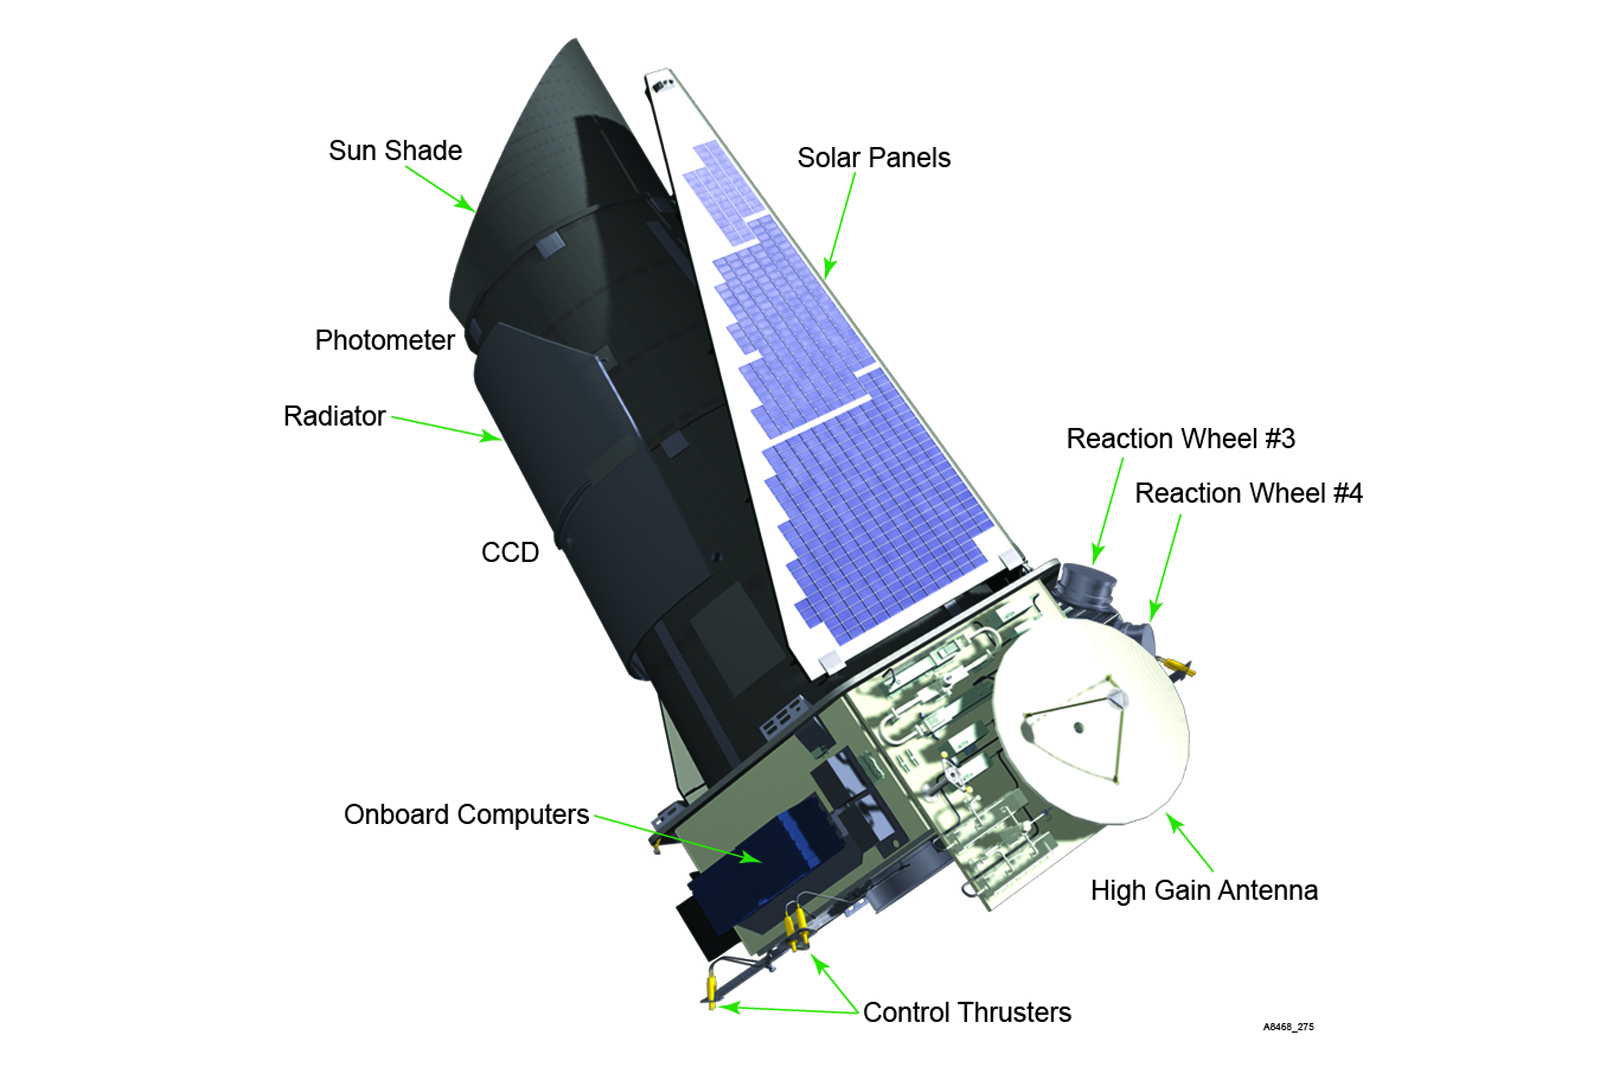
\includegraphics[width=0.6\textwidth]{images/750603main_Ball_Kepler_A8468_275_lg}
        \caption{The Kepler Satellite \autocite{keplerReactionWheelUpdate}}
    \end{figure}
    \note{
        Survey a single region of the galaxy for several years
        Photometer - array of CCDs, sole instrument
        pixels -> 30-min long or 1-min short cadence
        on Earth, calibrate + convert to light curves or target pixel files

    }
\end{frame}

\begin{frame}
    \frametitle{Procedure}
    \begin{enumerate}
        \item<1-> Light curves for Kepler-6b and Kepler-12b were obtained from the NASA Exoplanet Archive.
        \item<2-> The light curves were cleaned by removing all non-finite data points.
        \item<3-> The flux in each light curve was normalized by dividing by the median to aid in detrending and periodogram generation.
        \item<4-> The light curves were detrended by using least-squares regression to remove global trends.
        \item<5-> A periodogram of each light curve was generated using the box-fitting least squares algorithm.
        \item<6-> The periodogram and light curve were plotted so that transits and periods could be observed.
    \end{enumerate}
\end{frame}

\begin{frame}
    \frametitle{Procedure}
    \begin{enumerate}
        \setcounter{enumi}{6}
        \item<1-> The best period was determined from the periodogram by locating the highest peak.
        \item<2-> The transit epoch, ingresses, and egresses were determined from the light curve and period.
        \item<3-> The transit depth was calculated using the calculated list of transits.
        \item<4-> The estimated planetary radius was calculated from the transit depth and the stellar radius as listed in the Extrasolar Planets Encyclopedia.
        \item<5-> The percent errors between observed and actual values of the radius and period were calculated.
    \end{enumerate}
\end{frame}

\section{Calculations}

\begin{frame}
    \frametitle{Epoch}
    \begin{align*}
        \text{phase1} &= \text{in1} / \text{nb}                                                                                                                                                        &  \text{epoch} &= t_0 + \text{phase1} \times \text{period} \\
        \text{in1} &=  ((( kepler6b.target.periodogram.values.in1|sigfigs )))                                                                                                                          &  \text{period} &= ((( kepler6b.target.periodogram.best_period|sigfigs ))) \\
        \text{nb} &= ((( kepler6b.target.periodogram.values.nb|sigfigs )))                                                                                                                             &  t_0 &= ((( kepler6b.target.light_curve.time[0]|sigfigs ))) \\
        \text{phase1} &= ((( kepler6b.target.periodogram.values.in1|sigfigs ))) / ((( kepler6b.target.periodogram.values.nb|sigfigs )))                                                                &  &= ((( kepler6b.target.periodogram.values.phase1|sigfigs ))) \\
        \text{epoch} &= ((( kepler6b.target.light_curve.time[0]|sigfigs ))) + ((( kepler6b.target.periodogram.values.phase1|sigfigs ))) \times ((( kepler6b.target.periodogram.best_period|sigfigs ))) &  &= \SI{((( kepler6b.target.periodogram.epoch|sigfigs )))}{\bjd}\\
    \end{align*}
    \note{The epoch here refers to the time of the first transit in the light curve.
    One of the values comupted by the BLS implementation used is the bin index of the start of the transit, in1. Dividing this by the number of bins
    ,nb, (an input to the algorithm) yields the phase of the start of the transit. The epoch is then computed using this phase, the period, and the time
    of the first data point in the light curve.}
\end{frame}

\begin{frame}
    \frametitle{Duration}
    \begin{align*}
        \text{duration} &= \text{period} \times q \\
        &= ((( kepler6b.target.periodogram.best_period|sigfigs ))) \times ((( kepler6b.target.periodogram.values.q|sigfigs ))) \\
        &= \SI{((( kepler6b.target.periodogram.duration|sigfigs )))}{\bjd}
    \end{align*}
    \note{The duration of the transit is calculated from the period and \(q\), the fractional transit duration.}
\end{frame}

\begin{frame}
    \frametitle{Ingress and Egress}
    \begin{align*}
        \text{ingress} &= \text{epoch} + \text{period} \times (n - 1) - 0.2                                                                                                                  &  & \\
        &= ((( kepler6b.target.periodogram.epoch|sigfigs ))) + ((( kepler6b.target.periodogram.best_period|sigfigs ))) \times 2 - 0.2                                                        &  &= \SI{((( kepler6b.target.periodogram.ingresses[2]|sigfigs(5) )))}{\bjd} \\
        \text{egress} &= \text{epoch} + \text{period} \times (n - 1) + \text{duration} + 0.2                                                                                                 &  & \\
        &= ((( kepler6b.target.periodogram.epoch|sigfigs ))) + ((( kepler6b.target.periodogram.best_period|sigfigs ))) \times 2 + ((( kepler6b.target.periodogram.duration|sigfigs ))) + 0.2 &  &= \SI{((( kepler6b.target.periodogram.egresses[2]|sigfigs(5) )))}{\bjd}
    \end{align*}
    \note{The ingress and egress times of the \textit{n}th transit can be calculated from the epoch, period, and duration. A margin of \SI{0.2}{\bjd} is added on either side.}
    \note{The calculations are for the 3rd transit}
\end{frame}

\begin{frame}
    \frametitle{Transit Depth}
    \begin{align*}
        \Delta F &= \frac{ F_{\text{no transit}} - F_{\text{transit}} }{ F_{\text{no transit}} } \\
        &= \frac{((( kepler6b.f_no_transit|sigfigs ))) - ((( kepler6b.f_transit|sigfigs )))}{((( kepler6b.f_no_transit|sigfigs )))} \\
        &= ((( kepler6b.transit_depth|sigfigs )))
    \end{align*}
    \note{The transit depth is defined in terms of the flux during and outside of a transit. Here the flux during transit is defined as the average of the
    flux values at the bottom of each transit and the flux outside of transit is defined as the average of the flux values not contained in a transit.}
\end{frame}

\begin{frame}
    \frametitle{Planetary Radius}
    \begin{align*}
        \Delta F &= (\frac{R_p}{R_*})^2                                                                                       &  R_p &= \sqrt{\Delta F} \times R_* \\
        \Delta F &= ((( kepler6b.transit_depth|sigfigs )))                                                                    &  & \\
        R_* &= \SI{((( kepler6b.target.star.radius|sigfigs )))}{\solarRadius}                                                 &  &= \SI{((( kepler6b.target.star.radius_meters|sigfigs )))}{\meter} \\
        R_p &= \sqrt{((( kepler6b.transit_depth|sigfigs )))} \times \num{((( kepler6b.target.star.radius_meters|sigfigs )))}  &  & \\
        &= \SI{((( kepler6b.planet_radius_meters|sigfigs )))}{\meter}                                                         &  &= \SI{((( kepler6b.planet_radius|sigfigs )))}{\jupiterRadius}
    \end{align*}
    \note{Usually, the radii of stars are given in terms of solar radii, where \(1 R_{\astrosun} = \SI{6.955e8}{\meter}\), and planetary
    radii are given in Jupiter radii, where \(1 R_J = \SI{7.1492e7}{\meter}\). However, radii are converted to meters when performing calculations
    involving the two.}
\end{frame}

\section{Data}

((* for planet in all_planets *))
\begin{frame}
    \frametitle{((( planet.target.name )))}
    \begin{figure}
        \centering
        \includegraphics<1>[width=0.8\textwidth]{((( planet.light_curve_image )))}
        \includegraphics<2>[width=0.8\textwidth]{((( planet.periodogram_image )))}
    \end{figure}
    \only<3>{
        \begin{tabu} to \textwidth {lrrr}
                                                   &  Measured                                                  &  Actual                                         & Percent Error                                         \\
            Orbital Period [\si{\day}]             & ((( planet.target.periodogram.best_period|sigfigs(4) ))) & ((( planet.target.truth.period|sigfigs(4) ))) & \SI{((( planet.period_err|sigfigs(4) )))}{\percent} \\
            Planetary Radius [\si{\jupiterRadius}] & ((( planet.planet_radius|sigfigs(4) )))                  & ((( planet.target.truth.radius|sigfigs(4) ))) & \SI{((( planet.radius_err|sigfigs(4) )))}{\percent}
        \end{tabu}
    }
\end{frame}

((* endfor *))
\note{
Kepler-6b is a good example of a more-or-less ideal light curve. Since there are only 3 transits, use it to show ingresses, egresses, and epoch.
Use Kepler-12b to show difficulties - gaps, less-uniform transit depths, multiple peaks in periodogram
}

\begin{frame}
    \frametitle{Conclusion}
    \begin{itemize}[<+->]
        \item Clear peaks
        \note{Especially on Kepler-6b, the best period is clearly the best}
        \item Visible transits
        \note{In my experience, short-duration transits are easier to see since they look like lines or V's instead of curves or U's}
        \item Expected to "find" planets
        \note{I chose systems with known single planets - test the method itself against known systems, since most "easy" exoplanets already found, humans can be better at pattern recognition}
        \item System parameters close
        \note{Within 1\% error for periods, 7\& error for radii - more calculations for radii}
    \end{itemize}
\end{frame}

\begin{frame}
    \frametitle{Sources of Error}
    \begin{itemize}[<+->]
        \item Gap in light curves
        \note{Kepler 12b around 1417 days - could mess with periodogram, transit depth since I could be missing a transit}
        \item Single light curve
        \note{Can't really stitch together curves since they aren't sequential, but that means less data, could miss something - e.g. Kepler-6 curve only about 10 days}
    \end{itemize}
\end{frame}

\begin{frame}
    \frametitle{Further Areas}
    \begin{itemize}[<+->]
        \item Multi-planet systems
        \note{I want to see if this could pick up periods for multiple planets, e.g. Kepler-32}
        \item Noisier transits
        \note{The transits for the planets I studied (and Kepler-5b in the picture) are fairly visible. What happens if the transits aren't as clear}
        \item Radial velocity comparison
        \note{Wanted to do this initially. There are some parameters, like period, that both can predict. If I do both, how well do the results agree?}
    \end{itemize}
\end{frame}

\ifbeamer@inpresentation
\begin{frame}[allowframebreaks]
    \frametitle{Bibliography}
    \nocite{*}
    \printbibliography
\end{frame}
\fi

\end{document}
